\chapter{Introduction}
\label{chap:Introduction}
\par\noindent
\textit{\textbf{Introduction}} This section describes the background and motivation of the research (section \ref{sec:Background}), the problem to be addressed (section \ref{sec:Problem}) and the proposed solution (section \ref{sec:Solution}).

\section{Background}
\label{sec:Background}
\par\noindent
In recent years, data science has become more and more prominent. Since large quantities of data have become omnipresent, big data processing is applicable in various fields of research and operations. This work focuses on the application of big data processing to railway system operations, more specifically the preconditions. Mainly, two areas show promise to benefit from big data usage, which is predictive maintenance as well as optimization of railway operations. As the name suggests, lots of data is required, think hundreds of terabyte for freight operations in Germany alone. As it stands though, unfortunately, this data source remains largely untapped today, owing to freight wagons typically lacking necessary sensory equipment. This is where this work comes into play.

\subsection{Railway Vehicle Operations}
\label{sec:RailwayVehicleOperations}
\par\noindent
Road and rail traffic are fundamentally different, mainly in two regards. First, the physical properties, which will be discussed in chapter \ref{chap:FundamentalsOfRailwayVehicleEngineering}, second, the actual modalities of operations, which will be topic of this section.
\par
In road traffic, there are many different vehicles, all operating independently from one another. Although there is ongoing experimentation to utilize autonomous vehicles to recreate train-like lorry configurations, this is not the norm. In contrast to that, the track guiding of wheels offered by rails enables the formation of trains possibly kilometers long, reducing labor cost, infrastructure usage and energy consumption. This, of course, calls for special safety measures to be taken, since higher speeds and payloads result in long braking distances. 

\begin{figure}[H]
	\centering
	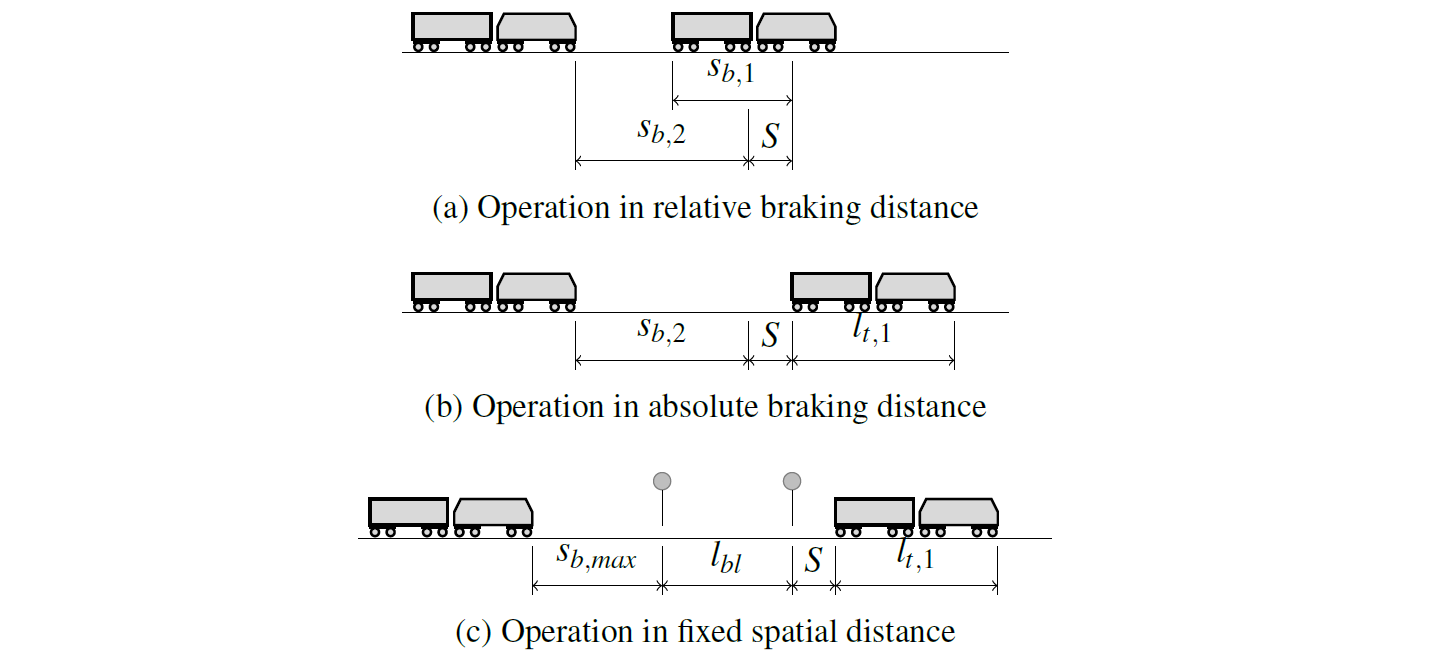
\includegraphics[width=\linewidth]{./pic/abstaende}
	\caption{Spacing paradigms \cite{Pfaff2017}}
	\label{fig:train_spacing}
\end{figure}

\par\noindent
Figure \ref{fig:train_spacing} illustrates the three main principles of spacing between two trains on the same track. $s_{b,i}$ denotes the braking distance of train $i$, $l_{t,i}$ the length of train $i$, $l_{bl}$ the length of a track section, and $S$ a safety margin. In fixed spatial distance, the distance between two trains must at least be the maximum braking distance $S_{b,max}$, plus the length of one track section (i.e. between two signals) $l_{bl}$, plus a safety margin $S$. In absolute braking distance, the distance between two trains must at least be the braking distance of the second train $S_{b,2}$, plus a safety margin $S$. Finally, in relative braking distance, the distance between two trains must be sufficient for the second train to be able to come to a full halt behind the first train if both trains start breaking at the same time. Fixed spatial distance, the most commonly used today, is very inefficient in terms of track utilization, but offers the most protection against accidents. In order to optimize efficiency, it is desirable to move towards relative braking distances, which requires the ability to very accurately predict braking capacity of trains.

\subsection{Automatic Train Protection and Cab Signaling}
\label{sec:ATPCS}
\par\noindent
Automatic train protection systems are designed to ensure safe operation in case of human or technical error or malpractice by the train operator. Generally, all trains operate on track sections which are free of other vehicles, reserved and locked. Think for example a section between two signals. These sections are also referred to as movement authority, and a train has to be capable of coming to a complete halt before the end of movement authority as to not violate a track section locked by another train. For this, the driver and/or the onboard computer needs to be informed about the endpoint of the current movement authority as well as speed limits. The train protection system enforces application of brakes in case of violation of restrictions, for example if the train exceeds the speed limit or the train would otherwise be unable to stop in time before movement authority expires. Train protection systems may be categorized by means of information transfer. Spatially discrete acting systems use transmitters placed at strategic points along the track, for example signals, whereas continuous systems may transmit information at all times, either via track-sided wire loops or radio communication. These allow higher degrees of automation than discrete systems, as trains have access to the necessary real-time data.
\par
Cab signaling relays all relevant information to the train operators so they may act in the most optimal way. The European train control system, short ETCS, encompasses both of these (\cite{Havryliuk2017}, p.12).

\subsection{Braking Curves}
\label{sec:BrakingCurves}
\par\noindent
For the ETCS to be able to supervise train velocity, it needs to determine the vehicle's braking capacity for any given moment in time, using a mathematical model of the braking dynamics and of the track characteristics. This prediction is called a braking curve, which describes the probable braking process for a set of input parameters. For an example, refer to figure \ref{fig:brakingcurves}. It shows a braking process, in particular the decline of the train's velocity over distance. Since braking performance cannot be predicted with absolute certainty, an $\epsilon$ parameter needs to be factored in to account for random behavior. Therefore, there is a number of discrete braking curves for any set of parameters, forming a probability distribution \cite{Pfaff2017}. The parameters may be classified in four categories:
\begin{itemize}
	\item Physical parameters, which are determined by real time measurements from on-board equipment
	\item Fixed values, like driver reaction time
	\item Trackside data, like track gradient or signaling data
	\item Train data, mostly captured beforehand, relating to the rolling stock braking system itself
\end{itemize}
The fourth category, train data, is the key factor for this work, as will be explained below.

\begin{figure}[H]
	\centering
	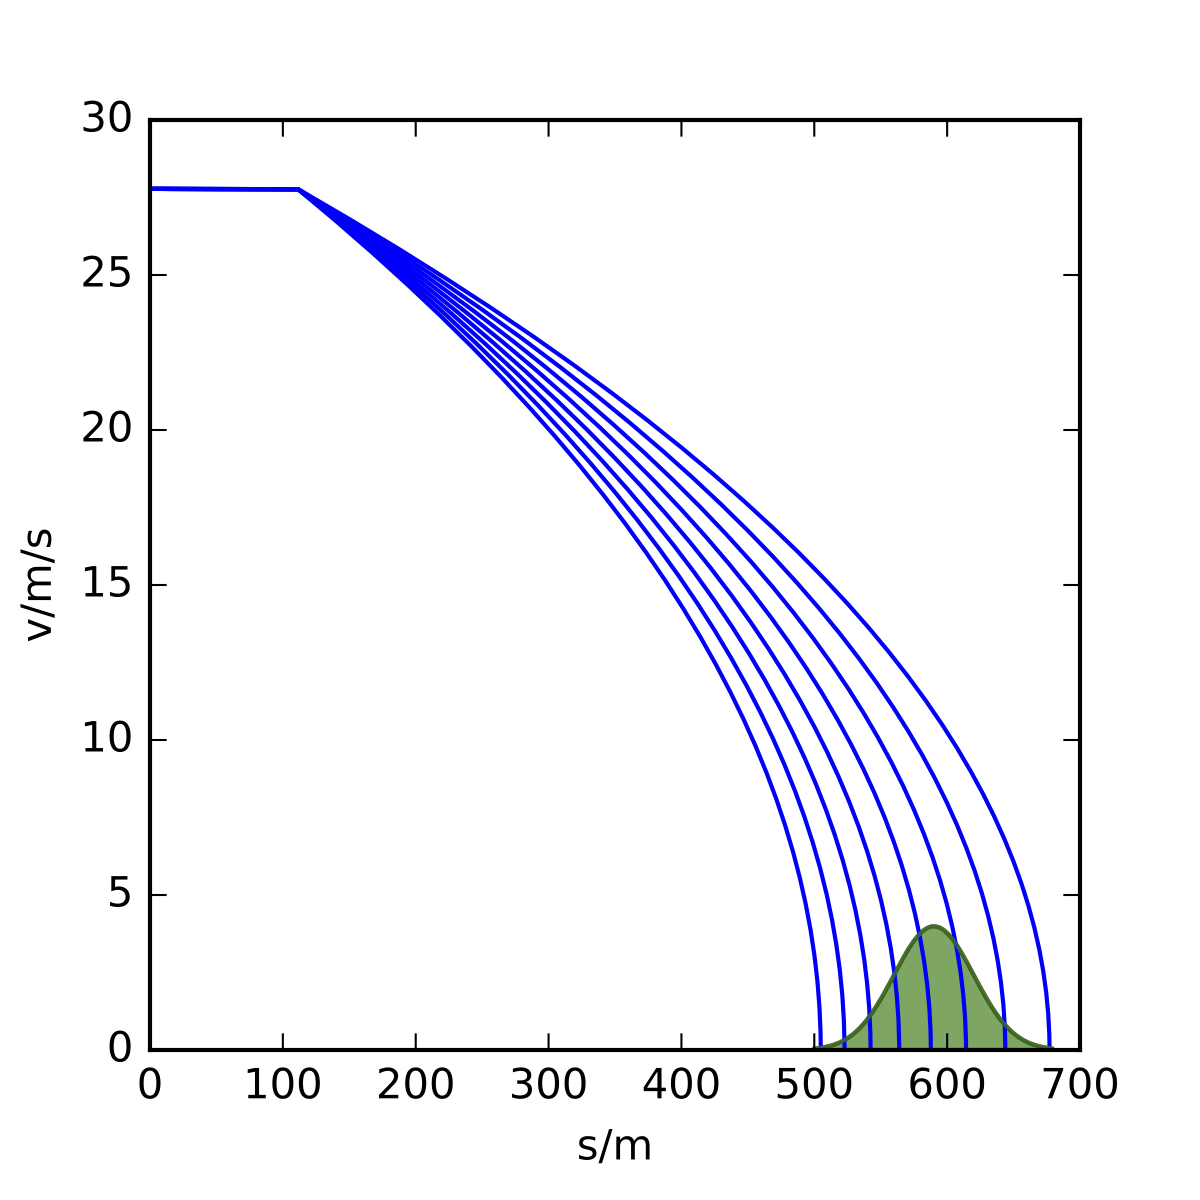
\includegraphics[scale=0.2]{./pic/171026_Transrail_BrakingCurves-14}
	\caption{Braking curves \cite{Pfaff2017}}
	\label{fig:brakingcurves}
\end{figure}

\section{Problem}
\label{sec:Problem}

\par\noindent
As mentioned, one category of input parameters for the calculation of braking curves is data directly associated with the rolling stock, and in particular to the braking system itself. While this does not necessarily present itself as an issue in passenger trains, freight wagons, in contrast, are usually not electrified and therefore do not currently posses the sensory equipment that would be necessary to obtain such data in an adequate quantity and quality, especially in regards to \textit{big data processing}. Although it has been proposed to equip freight wagons accordingly (Refer to the concept \enquote{freight wagon 4.0} by Dr. Manfred Enning and Dr. Raphael Pfaff \cite{Enning2017}), it will be years, possibly decades, before enough rolling stock has been retrofitted as to make it possible to obtain the desired data. Since braking curves vary according to the rolling stock, this lack of data makes calculation thereof impossible.

\section{Solution}
\label{sec:Solution}

\par\noindent
Since the problem is lack of data from real life operations, this work proposes to circumvent this by generation of artificial, simulated data instead. The data set should replicate the actual distribution of braking behavior as closely as possible. It is therefore necessary to first create a model encompassing the braking process of a freight train. This model will be discussed in depth in chapter \ref{chap:ModelingOfTrainOperations}. By using that model to run a large number of simulated braking processes, one may obtain data about the behavior of the braking system, which, albeit being artificial, should at least satisfy requirements for the calculation of rudimentary braking curves. A freely configurable simulation environment further allows for great flexibility in terms of input parameters, therefore enabling for covering a very large range of data, where computing power and time are the only limiting factors. The process of data generation and simulation will be discussed further in chapter \ref{chap:DataGeneration}.
\par
As real life operations would yield very high quantities of data, the simulation output must be stored in a data structure which is suitable for big data processing. This structure will also be discussed in chapter \ref{chap:DataGeneration}.